\section{Livello Data Link}
    \subsection{Trasmissione di stringhe}
        \problem
        Data la stringa di bit 0111101111101111110 che deve essere trasmessa a livello data link
        \begin{enumerate}
            \item Qual'è la stringa che viene effettivamente trasmessa dopo il \textit{bit stuffing}?
            \item Disegnare la \textit{codifica Manchester} della stringa trasmessa nell'esercizio pre\-cedente.
        \end{enumerate}

        \solution
        \begin{enumerate}
            \item Il bit stuffing prevede che si aggiunga uno 0 ogni cinque 1.
            
            \centerline{01111011111\underline{0}011111\underline{0}10}
            \item La codifica Manchester prevede che ogni 1 comporti una variazione dall'al\-to al basso e ogni 0 viceversa, pertanto ogni 0 verrà codificato come 01 e ogni 1 come 10.
            
            \centerline{011010101001101010101001101010101010}
        \end{enumerate}
    
    \subsection{Calcolo CRC}
        \problem
        Dovendo trasmettere la sequenza 110101 con metodo di rilevazione degli errori CRC a 2 bit con polinomio generatore 101 determinare le operazioni svolte dal trasmittente e dal ricevente.

        \solution
        Il trasmittente dovrà dividere la sequenza da inviare con due zeri accodati per il polinomio generatore 101, poi dovrà inviare la sequenza originale con il resto della divisione accodato.

        Il dato trasmesso è 110101\underline{11}.

        \begin{center}
    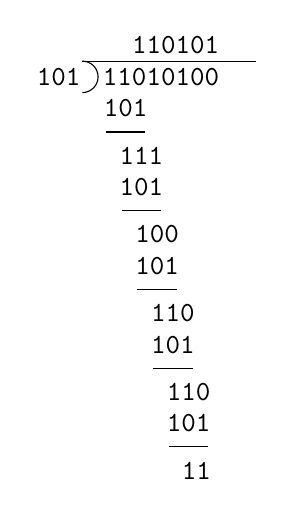
\begin{tikzpicture}
        % Intestazione
        \node at (1.185,0.2) {\verb:110101:};
        \node at (-0.3,-0.2) {\verb:101:};
        \draw (2.2,0) -- (0,0);
        \draw (0,-0.4) arc (90:270:-0.2);

        % Calcoli
        \node at (1,-0.2) {\verb:11010100:};
        \node at (0.55,-0.6) {\verb:101:};

        \draw (0.3,-0.9) -- (0.8,-0.9);
        \node at (0.75,-1.2) {\verb:111:};
        \node at (0.75,-1.6) {\verb:101:};

        \draw (0.5,-1.9) -- (1,-1.9);
        \node at (0.95,-2.2) {\verb:100:};
        \node at (0.95,-2.6) {\verb:101:};

        \draw (0.7,-2.9) -- (1.2,-2.9);
        \node at (1.15,-3.2) {\verb:110:};
        \node at (1.15,-3.6) {\verb:101:};

        \draw (0.9,-3.9) -- (1.4,-3.9);
        \node at (1.35,-4.2) {\verb:110:};
        \node at (1.35,-4.6) {\verb:101:};

        \draw (1.1,-4.9) -- (1.6,-4.9);
        \node at (1.45,-5.2) {\verb:11:};        
    \end{tikzpicture}
\end{center}

        Il ricevitore dovrà dividere il dato ricevuto per il polinomio generatore, se il risultato è diverso da zero c'è stato un errore durante la trasmissione.
    \subsection{Calcolo CRC Pt. 2}
        \problem
        Dovendo inviare la sequenza 101110 con CRC (polinomio generatore $x^3+1$):
        \begin{enumerate}
            \item Determinare la sequenza realmente trasmessa.
            \item Determinare le operazioni compiute dal ricevente nel caso in cui il terzo bit da sinistra viene invertito durante la trasmissione.
        \end{enumerate}

        \solution
        \begin{enumerate}
            \item \mbox{}\\\includegraphics[scale=0.6]{crc}
            \item da fare
        \end{enumerate}

    \subsection{Calcolo CRC Pt. 3}
        \problem
        Data la parola 10100111 da inviare con CRC-4  e il polinomio generatore 10111, determinare la sequenza inviata (Codeword) ed eseguire il calcolo del ricevente per verificare la correttezza del dato ricevuto.

        \solution
        \includegraphics{crc2}

    \subsection{Esercizio sulle finestre}
        \problem
        Si consideri una connessione  tra un client ed un server per l'upload affidabile di un file di dimensione O=256KB utilizzando il protocollo \textit{sliding windows}. \\
        Si supponga che:
        \begin{itemize}
            \item Il trasferimento avvenga tramite frame di dimensione pari a S=512 Byte.
            \item Non si verifichino errori di trasferimento o perdite di dati e che la finestra W rimanga costante.
            \item Il tasso di trasferimento rimanga costante e pari a R=32Kb/s.
            \item Il round-trip time tra client e server sia pari a RTT=200 ms.
        \end{itemize}
        
        Assumere che i tempi di trasmissione degli ACK siano trascurabili.
        
        Domande:
        \begin{enumerate}
            \item Disegnare il diagramma spazio-tempo del trasferimento
            \item Determinare la dimensione minima della finestra  W in byte per la quale si riesce a trasmettere dal server al client Frame senza interruzioni. 
            \item Determinare il tempo totale per il trasferimento completo del file.
        \end{enumerate}

        \solution
        \begin{equation*}
            T_{tr} = \frac{4096}{32 \cdot 10^3} = 128 ms
        \end{equation*}

        Numero bit che si possono inviare nel tempo RTT:
        \begin{equation*}
            200 \cdot 10^{-3} \cdot 32 \cdot 10^3 = 6400 ~ bit
        \end{equation*}

        Dobbiamo quindi poter inviare almeno 10496 (6400+4096) bit (1312 byte) senza attendere ACK

        Visto che i frame sono di dimensione fissa  dobbiamo arrotondare a 1536 byte (3 frames).

        Tempo complessivo: 128 ms $\cdot$ 500 frame + 1 RTT = 64,2 s
    
    \subsection{Rete Aloha}
        \problem
        Si consideri una rete ALOHA in cui i frame sono 200 bit con una velocità di 200kbps.

        Determinare il throughput (kbps) se il sistema produce 1000 frame/secondo nel caso di  Aloha puro e slotted.

        \solution
        $Tempo ~ di ~ frame = \frac{200}{200K} = 1ms$\\
        $Frame ~ per ~ tempo ~ di ~ 1 ~ frame: G = 1000 / 1000 = 1$\\
        Aloha Puro:
        $S = G \cdot e \cdot -2G = e-2 = 0,135$\\
        Throughput = 0.135 $\cdot$ 200 K b/s = 27 Kb/s\\
        Slotted Aloha: $S = G e -G =  e -1 = 0,367$\\
        Thoroghput = 0,367 $\cdot$ 200 k b/ s = 73,57 Kb
    
    \subsection{Probabilità di collisione}
        \problem
        Tre stazioni A, B e C condividono una LAN con algoritmo esponenziale binario per la gestione del Backoff e vorrebbero spedire un frame al prossimo slot.

        \begin{itemize}
            \item La stazione A inizia ora a trasmettere.
            \item La stazione B ha avuto 2 collisioni negli slot precedenti.
            \item La stazione C ha avuto una collisione.
        \end{itemize}

        Qual'è la probabilità di collisione al prossimo tentativo?

        \solution
        \begin{equation*}
            P_a = 1, ~ P_b = \frac{1}{4}, ~ P_c = \frac{1}{2}
        \end{equation*}

        A trasmette sicuramente; si ha collisione se trasmette anche b oppure c:

        \begin{equation*}
            P_b + P_c - P_b \cdot P_c = \frac{1}{4} + \frac{1}{2} - \left(\frac{1}{4} \cdot \frac{1}{2}\right) = \frac{5}{8}
        \end{equation*}

        (Devo sottrarre il caso di trasmissione contemporanea di b e c per evitare di contarla due volte)

        Un altro metodo è l'elencazione di tutti i casi:

        \begin{table}[H]
            \centering
            \begin{tabular}{c|c|c|c|c|c|c|c|c|c}
                \hline
                A & 1 & 1 & 1 & 1 & 1 & 1 & 1 & 1\\
                \hline
                B & 0 & 0 & 0 & 1 & 0 & 0 & 0 & 1\\
                \hline
                C & 0 & 0 & 0 & 0 & 1 & 1 & 1 & 1\\
                \hline
                & $\circ$ & $\circ$ & $\circ$ & $\times$ & $\times$ & $\times$ & $\times$ & $\times$ \\
                \cline{2-9}
            \end{tabular}
            \caption*{L'ultima riga mostra la probabilità pari a 5/8}
            \label{table:elenco}
        \end{table}